

\section{Set Encoding}
We have mentioned that, for flat tags, the number of forwarding table entries required for a single attribute test can be large. 
To understand the problem, let us consider a simple example for the case of attaching lists of anycast hosts to a packet. Say that there is a local area network with five hosts $H = \{h_1, h_2, h_3, h_4, h_5\}$, and each packet that arrives will be classified as anycasting to one of four possible host sets: $s_1 = \{h_1, h_2\}$, $s_2 = \{h_1, h_2, h_3\}$, $s_3 = \{h_1, h_3\}$, or $s_4 = \{h_3, h_4, h_5\}$. In a flat tagging solution to this problem, each unique set will be assigned a single tag, and thus a packet which can be forwarded to the $i^{th}$ set will receive the $i^{th}$ tag. Now, for an intermediate switch to determine, using exact tag matches, if a packet can be forwarded to host $h_1$, it must check whether the packet has been assigned to $s_1, s_2,$ or $s_3$. The number of entries required is proportional to the number of sets which contain $h_1$, in this case 3. In the worst case $h_1$ would be a member of almost every group, and testing for $h_1$ would required a number of checks linear in the number of tags. 


\subsection{Set Bitmasks}

For the sake of explanation, assume that it is possible to attach an arbitrary
amount of metadata to each packet the moment it is classified,
and that forwarding table entries are
able to read and write to this metadata arbitrarily. We can easily use this hypothetical
metadata to test for membership of any attribute. If there are $N$ possible attributes, we can write $N$ bits to the
metadata: the $i^{th}$ bit corresponds to the $i^{th}$ attribute. The moment the packet is classified, the $i^{th}$ bit is set to 1 if the $i^{th}$ attribute is true for that flow, and 0 if it is not. As a result, if we wish to test for the presence of attribute $x$, we need only check that $x$'s bit is 1 in the metadata before rerouting, rather
than exact matching on every tag that contains $x$.

Of course, we cannot attach arbitrary metadata to packets. Rather, we can repurpose a field in the header for tagging. In FlowTags, the Fragment Identification field is used. In SDX, the destination MAC stores the tags. In both cases, there is a hard limit on the size of tags to at most a few bytes. The scheme of creating a bitmask to encode a set of attributes will fail the moment the universe of attributes grows too large. This further motivates our optimized encoding scheme for reducing both memory usage and tag width.


\subsection{Multiple Masked Sets}

 As our scheme currently stands, we are assigning a single bit of the metadata bitmask to every
attribute in the universe of attribute. If we have more attributes than bits in the header field used for tagging, this approach immediately fails.

The purpose of the metadata bitmask attached to each packet is to concisely convey whether each attribute is attached to that flow or not. The bitmask can be thought of as recovering the desired list of attributes by masking some \textit{superset} which contains all possible attributes. 

\begin{figure}[t!] 
\begin{minipage}{1\linewidth}
\begin{subfigure}[b]{0.96\linewidth}
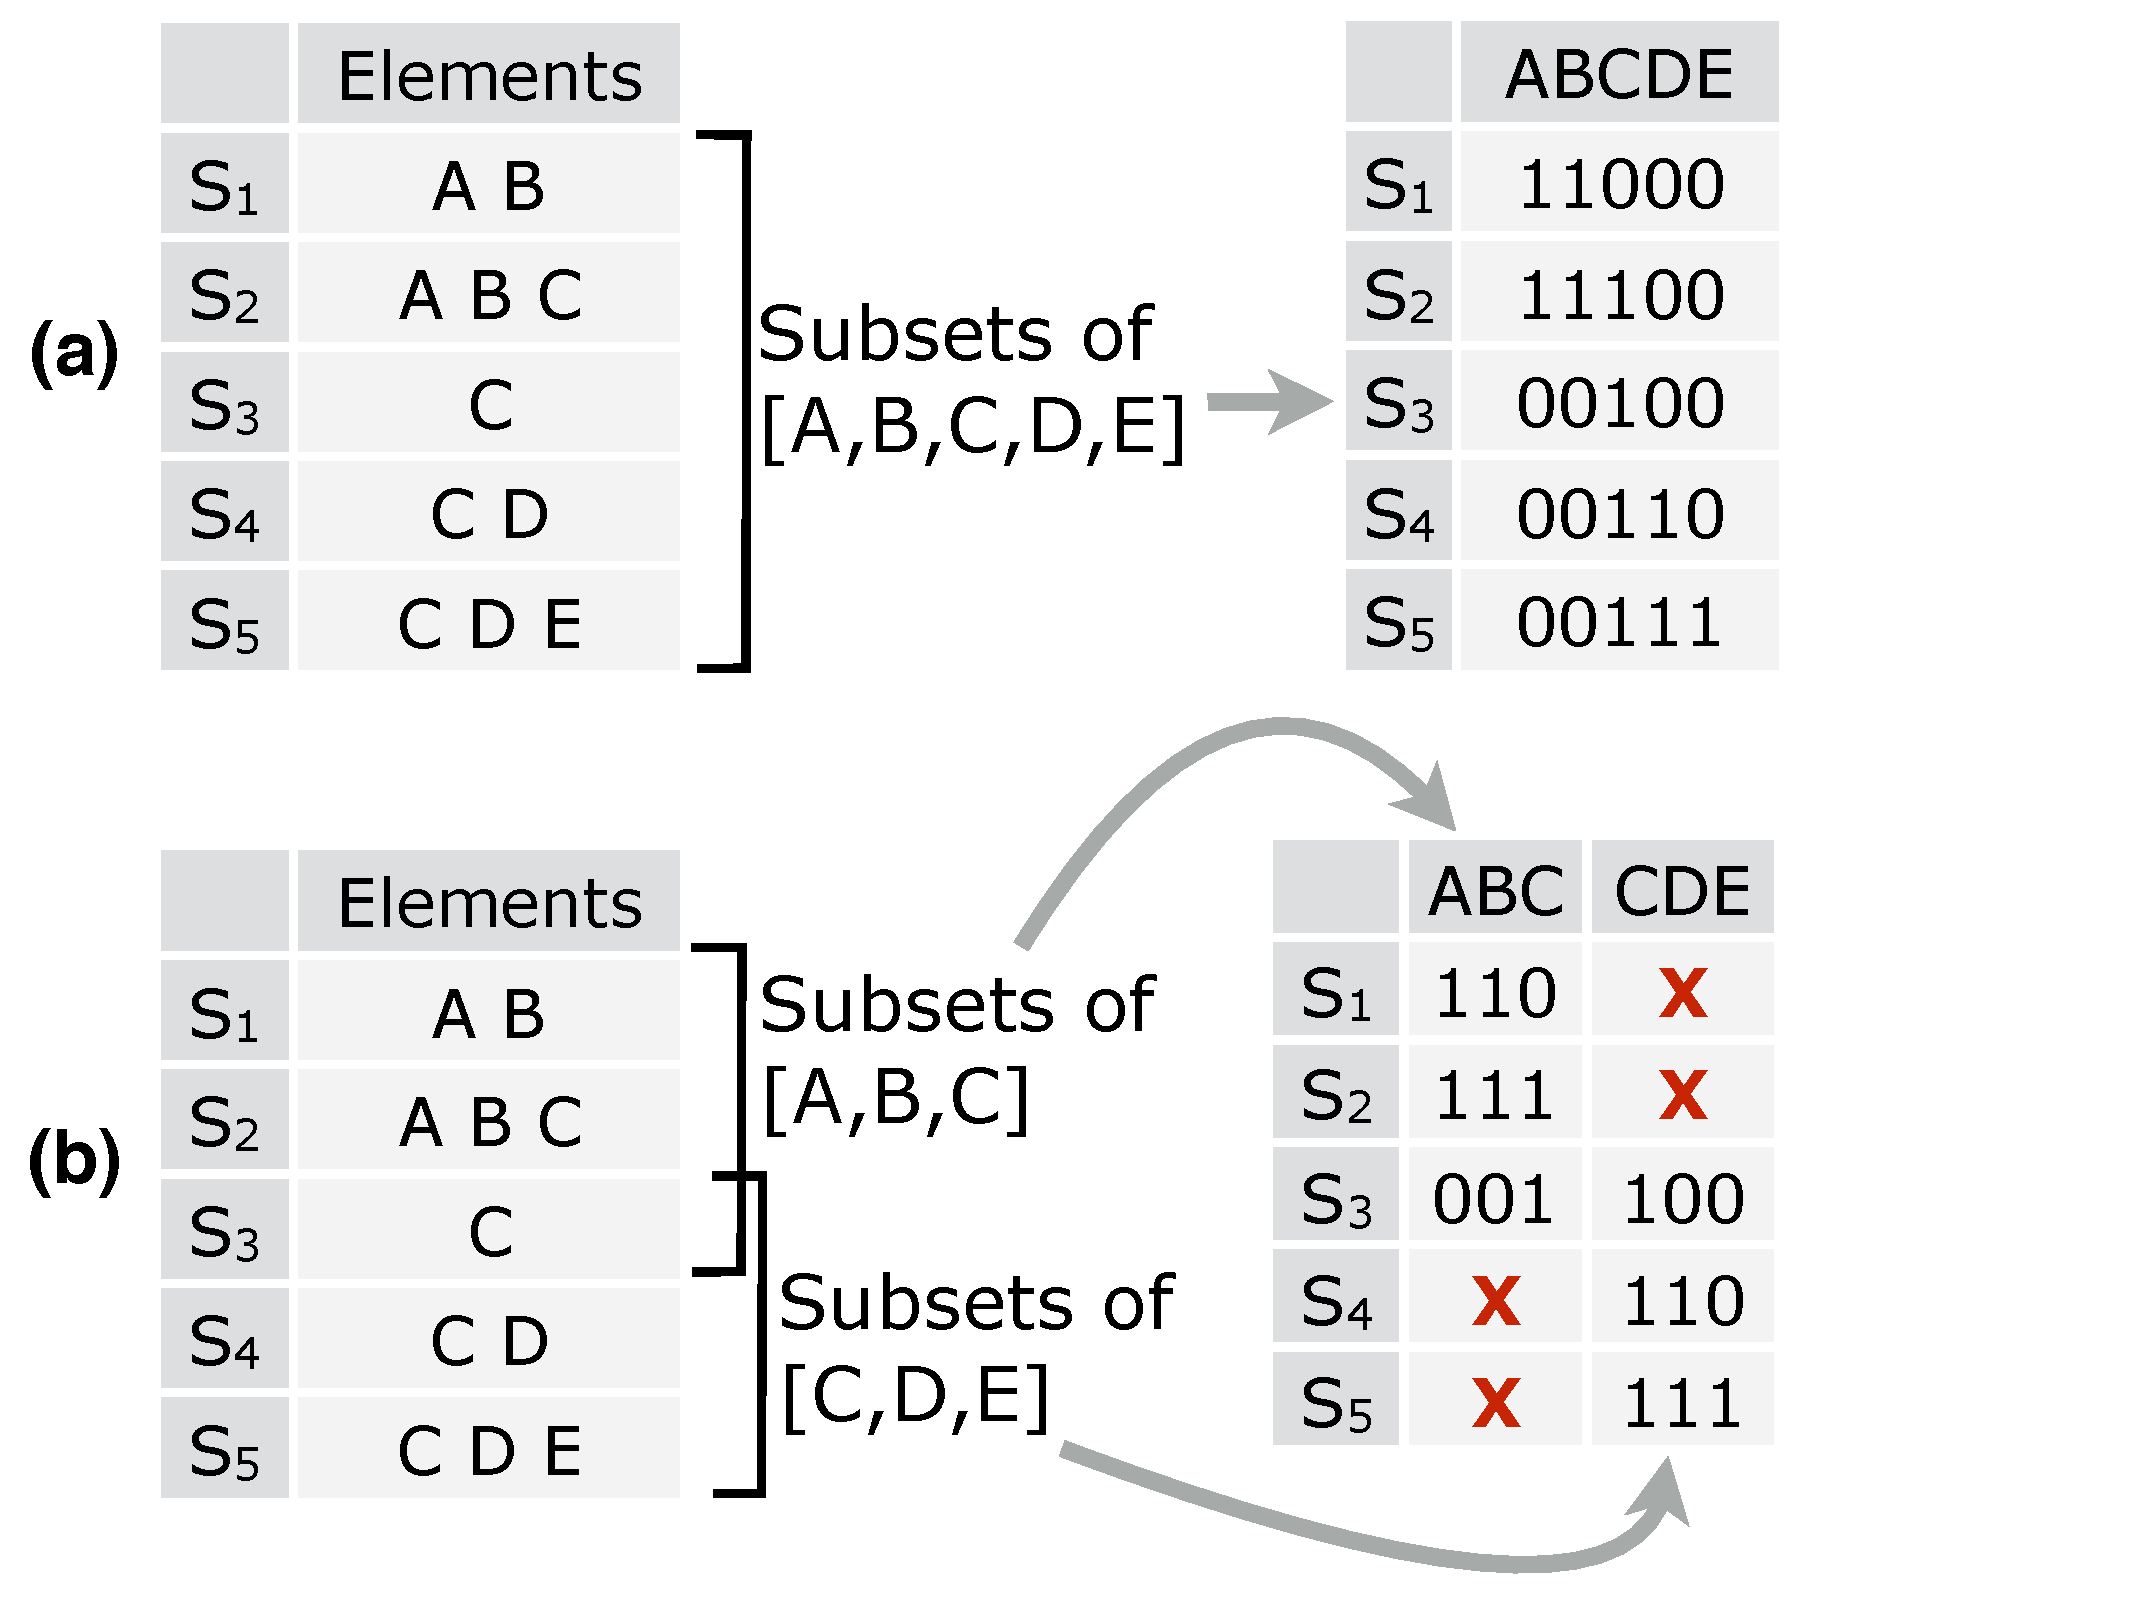
\includegraphics[trim={0 0 5.5cm 0}, clip, width=\linewidth]{figures/masking}
\end{subfigure} 
\begin{subfigure}[c]{0.96\linewidth}
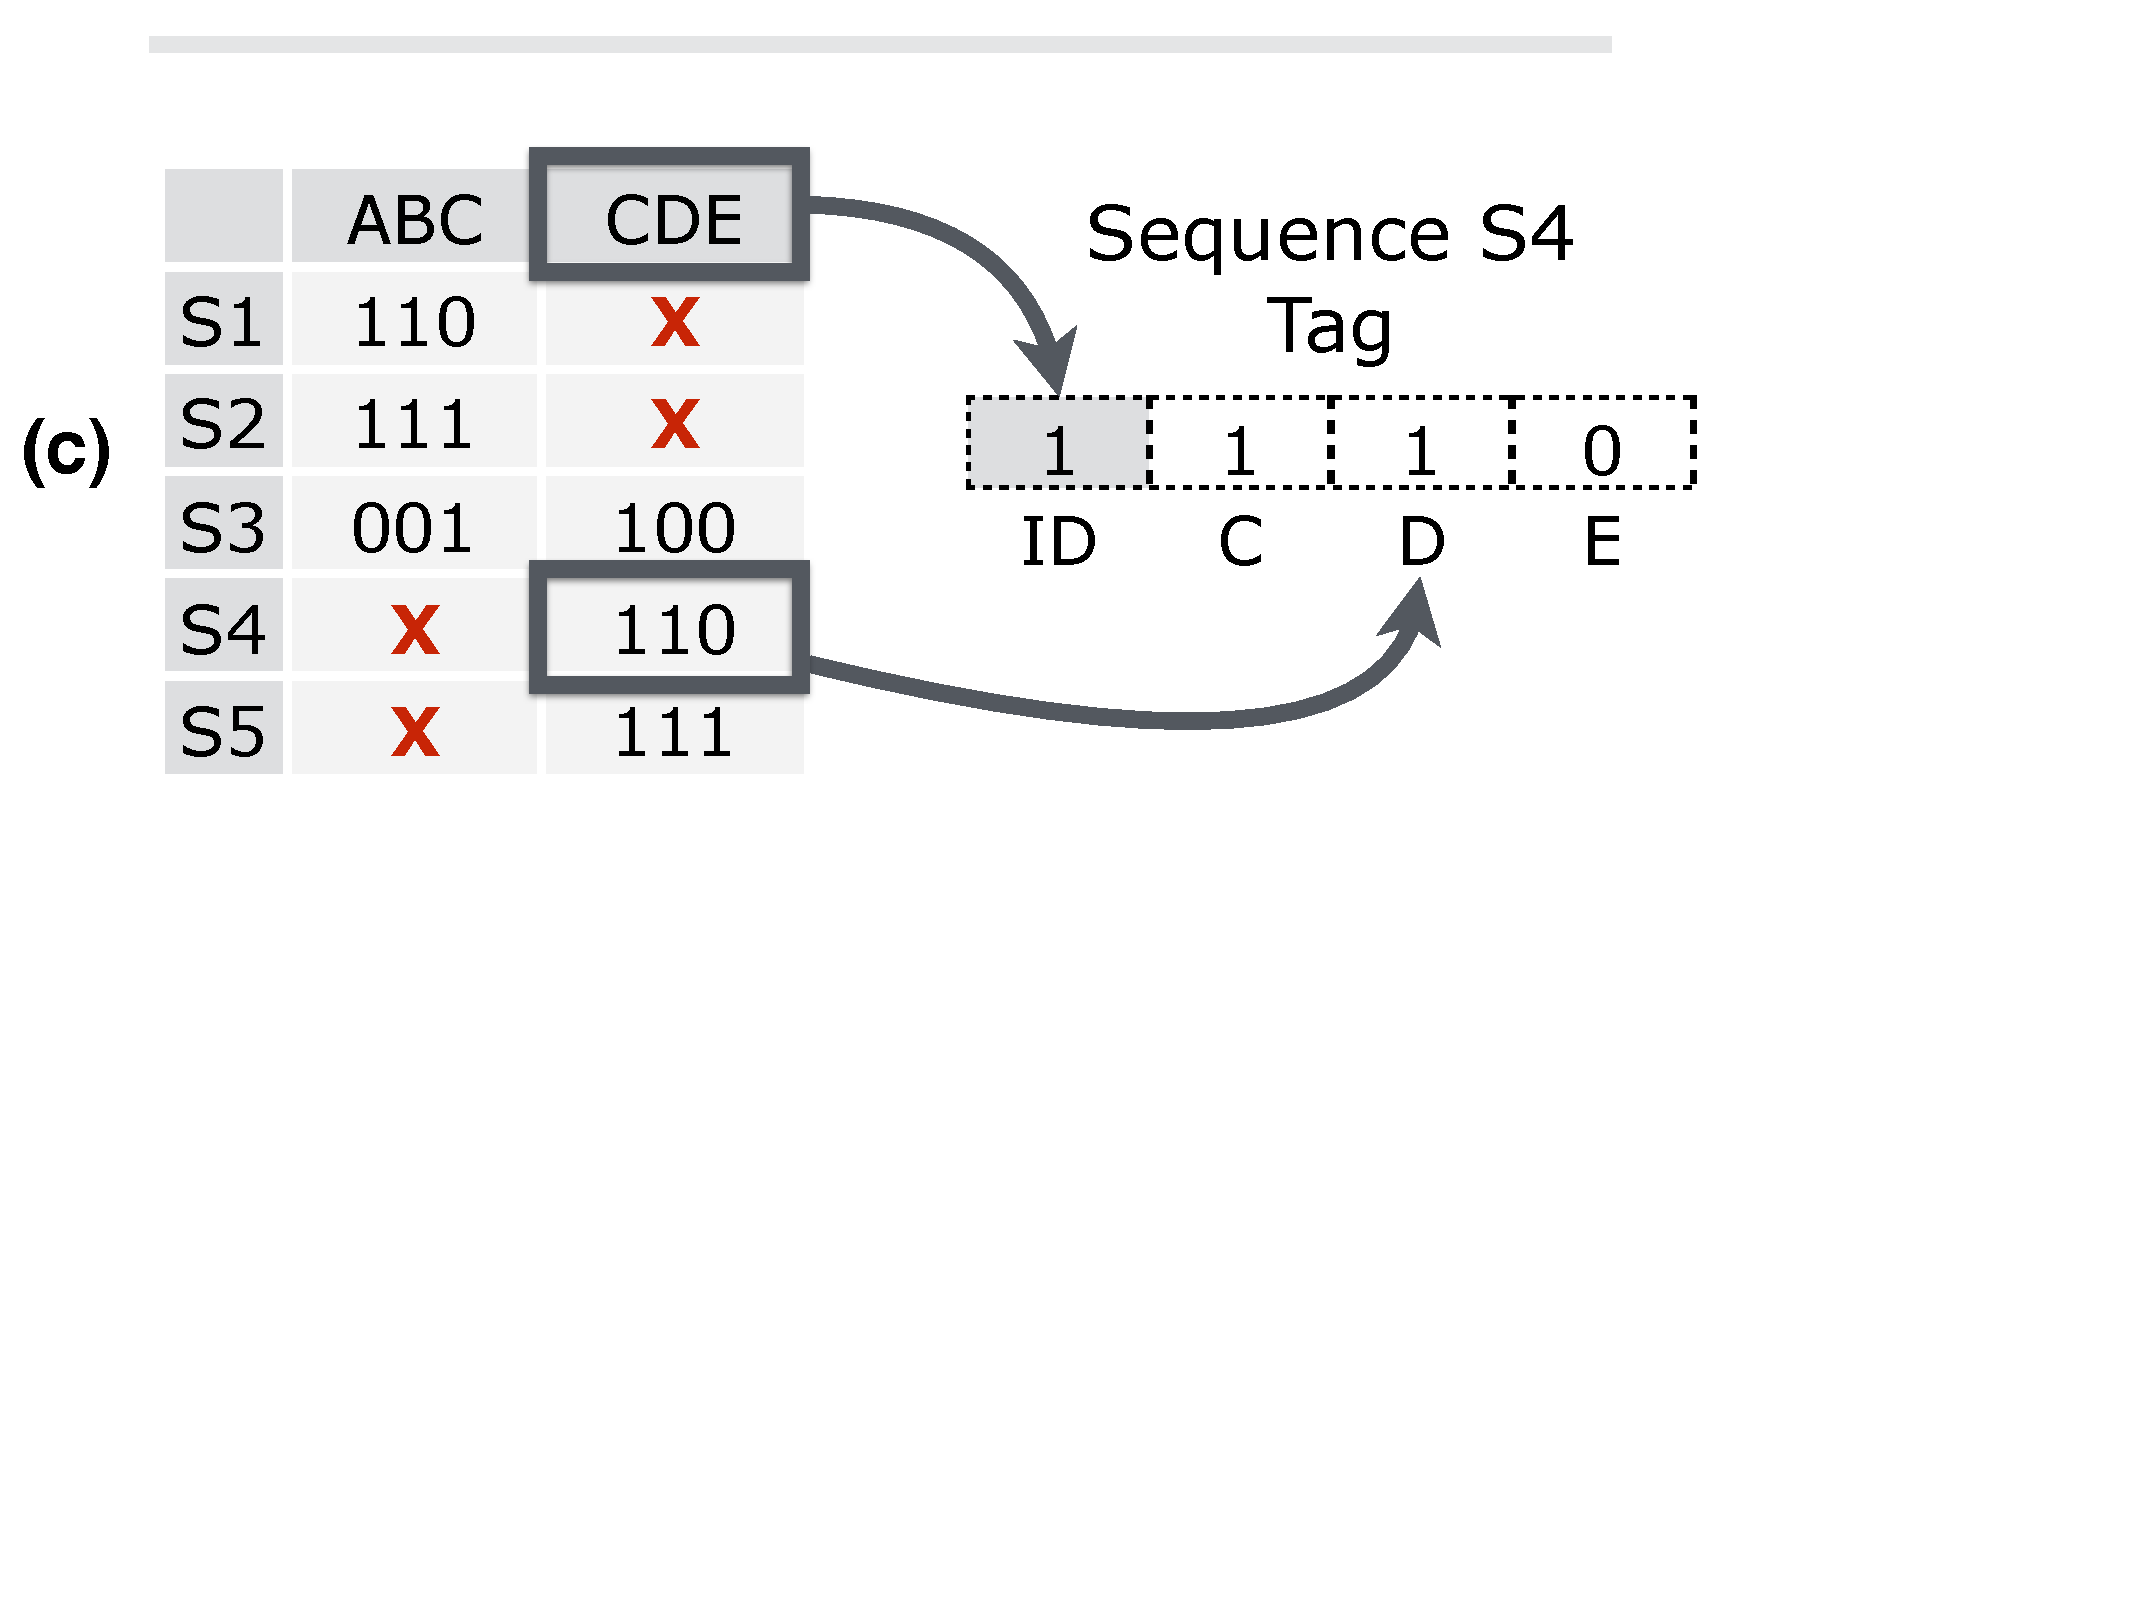
\includegraphics[trim={0 13cm 5.5cm 0}, clip, width=\linewidth]{figures/making_metadata}
\end{subfigure} 
\end{minipage} 
\caption{This figure demonstrates two different ways to recover attribute sets. In (a), the sets are recovered by masking over $[A,B,C,D,E]$. In (b), the sets are recovered by masking over either superset $[A,B,C]$ or set $[C,D,E]$. An X denotes that the set cannot be fully recovered by masking over the given set. (c) shows how, if each superset is identified by a binary integer, each set can be converted to a tag consisting of an identifier and a bitmask.}
\label{fig:masking}
\end{figure}

Consider the example in figure \ref{fig:masking}(a), where the left matrix contain the lists of attributes that we wish to recover, and the right matrix shows the bitmasks we would currently generate, which have a width of 5. Figure \ref{fig:masking}(b) shows that the attributes can be broken up into two categories: those which can be generated by masking over the superset $[A,B,C]$, and those which can be generated by masking over $[C,D,E]$. If we can add to our tag an identifier of the superset over which we are masking, we can have a reduced mask size! As shown in figure \ref{fig:masking}(c), if superset $[A,B,C]$ is identified as superset $0$, and $[C,D,E]$ is identified as superset $1$, then the tag for a packet $p_4$ which is mapped to set $[C,D]$ becomes $1110$, which is shorter than simply masking over the complete universe.

Now, if a switch wishes to test for attribute $D$, it must simultaneously check (1) the identifier for the superset that contains $D$ and (2) the bit in the bitmask which corresponds to $D$. Thus, the check that would be generated is\\
\noindent
{%\footnotesize
$\texttt{tag=1*1*} \rightarrow \texttt{action}(A)$\\
}
Where the first bit in the tag match is for the superset identifier, and the
remainder is for the mask.

However, looking again at figure \ref{fig:masking}(b), the case of testing for $C$'s membership is not so simple. Since $C$ appears in both supersets, we must check whether $C$'s bit is 1 in either superset mask. For example, if we had the rule\\
\noindent
{%\footnotesize
$\texttt{C in tag} \rightarrow \texttt{action}(A)$\\
}
This would be augmented under our scheme to become\\
\noindent
{%\footnotesize
$\texttt{metadata=0**1} \rightarrow \texttt{action}(A)$\\
$\texttt{metadata=11**} \rightarrow \texttt{action}(A)$\\
}
Therefore, depending upon the matrix construction, membership tests may still require multiple TCAM entries. If no superset is too large to fit into the mask, it is feasible to merge columns of the matrix to create new, larger supersets which can decrease the inflation factor. However, this can only be performed until the supersets of each column become too large to fit into the available bit space. For example, in figure \ref{fig:masking}(b), the two columns could be merged into $[A,B,C,D,E]$ to eliminate the inflation of $C$ rules. This would decrease the identifier size from 1 to 0 bits and increase the mask size from 3 to 5 bits. There is a 
tradeoff to consider between the size of the superset identifier, the mask size, and the number of rules for attribute testing, and when considered formally an optimization problem arises.

